\usepackage{amsmath}\documentclass{article}[12pt]

\usepackage{amsmath}
\usepackage{graphicx}
\usepackage{float}
\usepackage{listings}

\lstset{
    basicstyle          =   \sffamily,
    keywordstyle        =   \bfseries,
    commentstyle        =   \rmfamily\itshape,
    stringstyle         =   \ttfamily,
    flexiblecolumns,
    numbers             =   left,
    showspaces          =   false,
    showstringspaces    =   false,
    captionpos          =   t,
    frame               =   lrtb,
}

\lstdefinestyle{Python}{
    language        =   Python,
    keywordstyle    =   \color{blue},
    keywordstyle    =   [2] \color{teal},
    stringstyle     =   \color{magenta},
    commentstyle    =   \color{red}\ttfamily,
    breaklines      =   true,
    columns         =   fixed,
    basewidth       =   0.5em,
}

\author{490005761 lyu0226}
\title{COMP5329: Assignment1\\Report}

\begin{document}
\maketitle

\section{Introduction}\label{sec:introduction}
\subsection{Aim of study}\label{subsec:aim-of-study}
    The aim of this study is to understand the fundamentals of deep learning by implementing
    simple multilayer perceptron neural networks and related functions such as optimizers,
    activation functions and loss functions.
\subsection{Importance of study}\label{subsec:importance-of-study}
    The importance of this study is that the best way to learn the principles of deep
    learning is to practice them.

    However, mature frameworks often hide the process and methods of implementation
    from the user, wrapping complex processes in simple interfaces.Calling these
    encapsulated interfaces does not allow people to understand the principles,
    but merely to become "skilled interface users".
    Once a problems arises, When a problem arises, those who do not understand
    the principles are often unable to locate the root cause of the problem,
    or to deduce how to optimise the model by modifying hyperparameters.

    In this study, by implement an independent deep learning framework, subjects will obtain a
    better understanding towards the underlying principle of deep learning, and thus become a better
    problem solver in deep learning area.

\section{Methodology}\label{sec:methodology}
\subsection{Preprocessing}\label{subsec:preprocessing}
\subsubsection{Data Overview}\label{subsubsec:data-overview}
    The given data set is in shape of $(50000, 128)$, with a label of single integer value (0-9).
    The feature data has a standard deriviation of $1.1688637$ and mean $-1.59374025$.
    From the data quality perspective, the standard deriviation is very close to 1 and mean is close to 0,
    which is pretty good for model training.

    For the label data, the ground truth of samples are perfectly distributed.
    There are 10 classes in total, $50000$ samples, and $5000$ samples for each class precisely.

\subsubsection{Preprocess the Feature Data}
    Although the standard deriviation and mean of the feature data is good, there is still room for improvement.
    Before training, the feature data was standardized to 0 mean and standard deriviation 1 using the following method:
\[ x_{Standardized} = \frac{x - \mu}{\sigma} \]
    Where $\mu$ stand for mean of x and $\sigma$ is the standard deriviation of x.

\subsubsection{Preprocess the Label Data}
    The label data is in form of (0-9), which is numerically continuous but discrete in meaning.
    To make it able to be feed into the model, it must be encoded.
    Before training, the label data was one hot encoded from single integer to a 10 element vector.
    For example:

    \[ OnehotEncode([0, 1, 2]) = [[1, 0, 0], [0,1,0],[0,0,1]] \]

\subsection{Design}\label{subsec:design}
The best model is designed with 3 hidden layer, with 64, 32, 10 neuron seperately, initialized by
    Xavier Normal initialization.
    Each hidden layer is followed by a batch-normalization layer and a dropout layer with drop rate 0.25.
    Activation function is ReLU. Specifically, for last layer, the activation function is Softmax.
    Optimizer is Adam with momentum $\beta_1 = 0.9$ $\beta_2 = 0.999$,
    learning rate $1e-3$ and weight decay $0.02$.
    Loss function is Cross Entropy.

\subsection{Performance}
    The best model has obtained 0.5301 accuracy on testset meanwhile 0.1408 loss on trainset.
    For this result, the model has been trained for 91 epoch in 4min 28s on the test platform with
    Intel i9-9900K CPU @ 3.60GHz, Windows 11 OS, python 3.8.11, Numpy 1.22.3 and Scipy 1.8.0 through Jupyter lab 3.3.2.
    No other package or accelerator involved.
    In the further section, the experiments were performed on this platform as well.
    The best result given above was obtained at epoch 70.

\subsection{Module}\label{subsec:module}

\subsubsection{Layer}
    In a multilayer perceptron, the hidden layer is the fully connected layer.
    Its role is to take the features of the input data and abstract them into another dimensional space
    to reveal its more abstracted features, which can be better divided linearly.
    Multiple hidden layers are multiple levels of abstraction of the input features to achieve a better linear division.

    The layer keeps multiple neurons, each one contains two variable, weight and bias.
    Each neuron for each input $X$, it does:
\[ w^T X+b\]
    For a well-trained model, each neuron can be activated by a specific combination of features,
    outputting a strong signal to the next layer, thus contributing to the final result.

\subsubsection{Batch-normalization}
    Batch-normalization layer is to normalize the batch data during the training process.
    This layer will compute a moving average of mean and standard deriviation of output from previous layer,
    and normalize them to reach 0 mean and 1 standard deriviation.

\begin{gather*}
    \mu_{t} = \mu_{t-1} * (1-momentum) + momentum *\mu\\
    \sigma_{t} = \sigma_{t-1} * (1-momentum) + momentum *\mu\\
    Normalized_{t} = \frac{input_{t} - \mu_{t}}{\sigma_{t}}
\end{gather*}

    After normalization, the batchNorm layer will also do a shifting like hidden layer:

\[ out_{t} = \gamma Normalized_{t} + \beta \]

    Where $\gamma$ and $\beta$ are also trainable.

\subsubsection{Dropout}
    The dropout layer is used to make the output of the hidden layer sparse and reduce the complex co-adaptation
    relationship between neurons, thus reducing the probability of overfitting the model.

    The principle of it is to randomly set neurons' output to zero.
    The probabilty of this zerolization is user-defined.

\subsubsection{ReLU}
    ReLU, Rectified Linear Unit, is a kind of activation.
    It works by non-linearly transforming the linear output of each layer, so that the whole model becomes non-linear
    and more complex decision boundaries can be formed.

    It works by zeroing out negative numbers in the output of the previous layer,
    leaving values greater than or equal to zero as they are.

\subsubsection{Softmax}
    Softmax maps some inputs to real numbers between 0 and 1, and normalizes them to ensure that the sum is 1.
    It is designed to be used for multiple classification tasks, since the probability of multiple classes also sums to 1.

    For the input $V = [V_1, V_2, \dots V_j]$:
\[ Out_i = \frac{e^{V_i}}{\Sigma^i_j e^{V_i}}\]

\subsubsection{Adam}
    Adam optimization is a stochastic gradient descent method that is based on adaptive estimation of first-order and
    second-order moments.
    Effective control of the learning rate step and gradient direction through first and second order momentum,
    preventing oscillation of the gradient and stationarity at the saddle point.

    If weight decay is defined, the gradient will be added by the $W * decayRate$ before updating.

\[g_t = g_t + W_{t-1} * decayRate\]

    First order moment: a moving average of gradient.

\[m_t = \beta_1 * m_{t-1} + (1 - \beta_1) * g_t\]

    Second order moment: a moving average of squared gradient.

\[V_t = \beta_2 * V_{t-1} + (1 - \beta_2) * g_t^2\]

    After the moments were computed, update the variable

\[W_t = W_{t-1} - \frac{lr * m_t}{\sqrt{V_t}}\]

\subsubsection{CrossEntropy}
    CrossEntropy loss function is designed to evaluate the prediction performance in multi-classification task.
    Its derivative is directly depends on the prediction and ground truth, thus it will be a very good loss function
    when the model is performing bad.
    But for a better model, the learning speed will decrease.

    For prediction $p$ and ground truth $y$:

\[ L = \frac{1}{N} \sum_i L_i  = -\frac{1}{N}\sum_i \sum^M_{c=1} y_{ic} \log(p_{ic}) \]

    Where $M$ indicates the total class number and $c$ stand for each class.

\section{Experiments and Results}\label{sec:experiments-and-results}
    To explore the best model, various hyper-parameter has been attempted.
    Following tests are performed with an Early-Exit Pipe which will stop the training process
    when the metric does not come better in certain rounds,
    (See detail at appendix or dl.utils.EarlyStopping.EarlyStoppingPipe) thus the total epoch may vary.

    A set of hyper-parameter has been selected at the begining the test.
\begin{itemize}
    \item Hidden Layer number: 3
    \item Batch size: 128
    \item Preprocessing: Standardization
    \item Optimizer: SGD
    \item LR: 1e-3
    \item Initialization: Kaiming normal initialization
    \item BatchNorm: Yes
    \item Dropout: 0.25
\end{itemize}
    After a set of comparison or ablation studies, the best set of hyper-parameter will be selected.

    To measure the performance, we have the metrics of training loss, training accuracy, test loss and test accuracy.
    The training accuracy and test loss does not mean a lot, and since this is a classification task, thus the test
    accuracy will be the metric which has been weighted the most.

\subsection{Hidden Layer}
    In this experiment, the models with 2, 3, 4 hiddenlayers will be evaluated.

\begin{table}[H]
    \centering
    \begin{tabular}{|c|c|c|c|}
        \hline
        Hidden Layer & Test Accuracy & Epoch & Time Cost/s\\\hline
        2 & 0.4846 & 33 & 101.91\\\hline
        3 & 0.5068 & 18 & 89.39\\\hline
        4 & 0.4891 & 72 & 331.5\\\hline
    \end{tabular}
    \caption{Performance of different hidden layer number}
\end{table}

\begin{figure}[H]
    \centering
    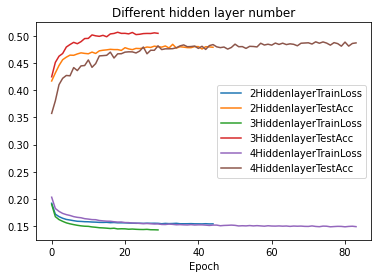
\includegraphics[scale=0.5]{Figures/1.Hiddenlayers/download}
    \caption{Performance of different hidden layer number}
\end{figure}

    As observed, 3 hidden layer obtained both fast training and higher accuracy.

\subsection{Batch Size}
    In this experiment, batch size of 64, 128, 256 has been tested. Result as below:

\begin{table}[H]
    \centering
    \begin{tabular}{|c|c|c|c|}
        \hline
        BatchSize & Test Accuracy & Epoch & Time Cost/s\\\hline
        64 & 0.5168 & 54 & 199.2629\\\hline
        128 & 0.5109 & 23 & 74.8191\\\hline
        256 & 0.5073 & 18 & 52.7593\\\hline
    \end{tabular}
    \caption{Performance of different batch size}
\end{table}

\begin{figure}[H]
    \centering
    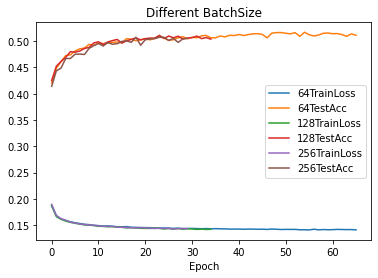
\includegraphics[scale=0.5]{Figures/2.BatchSize/download}
    \caption{Performance of different batch size}
\end{figure}

    As observed, batch size does not significantly affect the model performance.
    However,the training time seems like sensitive to it.
    Batch size 128 model has stopped converging
    at the very beginning, but the 64 batch size was osillating until 3 times of 128's best epoch.

    Although batch size 64 has obtained the best performance, but it's not significant
    and a huge over-cost on training time.
    To sum up, 128 would be the best batch size.

\subsection{Preprocessing}
    Pre-processing the data can often lead to positive feedback.
    However, given that the distribution of the original data is already good,
    pre-processing may still have negative effects.
    The result of raw data and standardized data as below:

\begin{table}[H]
    \centering
    \begin{tabular}{|c|c|c|c|}
        \hline
        Preprocessing & Test Accuracy & Epoch & Time Cost/s\\\hline
        Standardized & 0.5115 & 28 & 158.7205\\\hline
        Raw & 0.5188 & 40 & 151.399\\\hline
    \end{tabular}
    \caption{Performance of different preprocessing}
\end{table}

\begin{figure}[H]
    \centering
    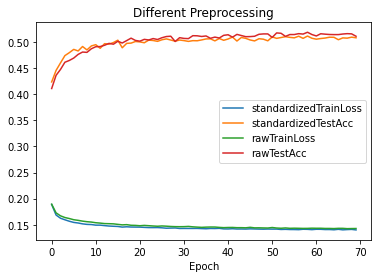
\includegraphics[scale=0.5]{Figures/3.Preprocessing/download}
    \caption{Performance of different preprocessing}
\end{figure}

    It can be observed that there is no significant difference on performance
    between the models trained by raw data or the standardized data.

    This is speculated to be because the distribution of the original data is already good.
    So in this task, the original data will be chosen for training.

\subsection{Optimizer}

    In this experiment, the different optimizers will be test, which are Adam and SGD.

\begin{table}[H]
    \centering
    \begin{tabular}{|c|c|c|c|}
        \hline
        Optimizer & Test Accuracy & Epoch & Time Cost/s\\\hline
        SGD & 0.5114 & 36 & 102.9382\\\hline
        Adam & 0.5231 & 40 & 160.5311\\\hline
    \end{tabular}
    \caption{Performance of different Optimizer}
\end{table}

\begin{figure}[H]
    \centering
    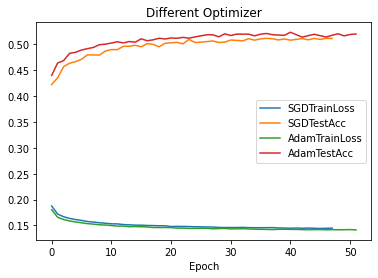
\includegraphics[scale=0.5]{Figures/4.Optimizer/download}
    \caption{Performance of different Optimizer}
\end{figure}

    As observed, Adam has a slightly better performance.

\subsection{Learning Rate}

    In this experiment, the model will be trained with 0.01, 0.001 and 0.0001 learning rate.

\begin{table}[H]
    \centering
    \begin{tabular}{|c|c|c|c|}
        \hline
        Learning Rate & Test Accuracy & Epoch & Time Cost/s\\\hline
        0.01 & 0.5018 & 39 & 162.8090\\\hline
        0.001 & 0.5266 & 91 & 254.2694\\\hline
        0.0001 & 0.5140 & 153 & 492.1130\\\hline
    \end{tabular}
    \caption{Performance of different Learning Rate}
\end{table}

\begin{figure}[H]
    \centering
    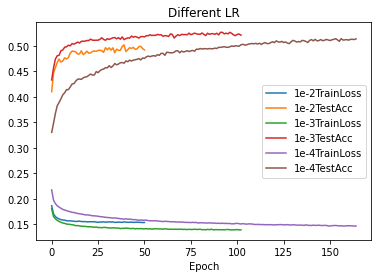
\includegraphics[scale=0.5]{Figures/5.LR/download}
    \caption{Performance of different Learning Rate}
\end{figure}

    As observed, a learning rate of 0.01 performs pretty bad.
    It stopped converging very early and did not reach an accuracy as high as the others.
    0.001 seems pretty good, with the best performance with a feasible converging time.
    As for 0.0001 lr, it takes too much time and did not reach the best performance.
    This is probably due to stucking in the local optimal.

\subsection{Initialization}

    In this experiment, various layer initializations will be evaluated.
    Include Xavier Normal/Uniform and Kaiming Normal/Uniform.

\begin{table}[H]
    \centering
    \begin{tabular}{|c|c|c|c|}
        \hline
        Initialization & Test Accuracy & Epoch & Time Cost/s\\\hline
        KaimingNormal & 0.5208 & 34 & 114.6010\\\hline
        KaimingUniform & 0.5154 & 34 & 142.7880\\\hline
        XavierNormal & 0.5239 & 61 & 206.2885\\\hline
        XavierUniform & 0.5236 & 46 & 139.4836\\\hline
    \end{tabular}
    \caption{Performance of different Initialization}
\end{table}

\begin{figure}[H]
    \centering
    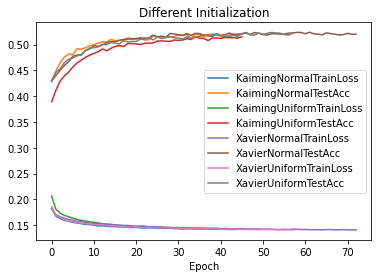
\includegraphics[scale=0.5]{Figures/6.initialization/download}
    \caption{Performance of different Initialization}
\end{figure}

    As observed, Xavier initializations are better than Kaiming in this task.
    The Xavier Normal is slightly better than the Xavier Uniform.

\subsection{Batch Normalization}

    To explore the influence of Batch Normalization, this experiment will evaluate the models with/without batchNorm.

    Result as follows:

\begin{table}[H]
    \centering
    \begin{tabular}{|c|c|c|c|}
        \hline
        BatchNorm & Test Accuracy & Epoch & Time Cost/s\\\hline
        With & 0.5241 & 64 & 203.3823\\\hline
        Without & 0.5248 & 84 & 252.7695\\\hline
    \end{tabular}
    \caption{Performance of models with/without BatchNorm}
\end{table}

\begin{figure}[H]
    \centering
    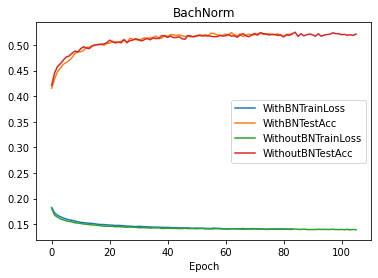
\includegraphics[scale=0.5]{Figures/7.BatchNorm/with-without bn}
    \caption{Performance of models with/without BatchNorm}
\end{figure}

    It can be observed for this task, bachnorm layers is not significantly affecting the performance.

\subsection{Dropout}

    To explore the influence of Dropout, this experiment will evaluate the models with/without Dropout.

    Result as follows:

\begin{table}[H]
    \centering
    \begin{tabular}{|c|c|c|c|}
        \hline
        Dropout & Test Accuracy & Epoch & Time Cost/s\\\hline
        With & 0.5224 & 81 & 245.4308\\\hline
        Without & 0.5247 & 13 & 71.3339\\\hline
    \end{tabular}
    \caption{Performance of models with/without Dropout}
\end{table}

\begin{figure}[H]
    \centering
    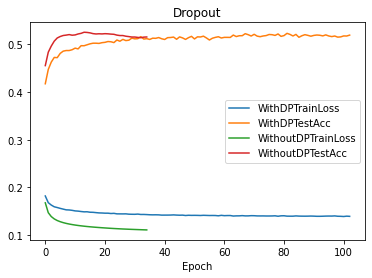
\includegraphics[scale=0.5]{Figures/8.dp/download}
    \caption{Performance of models with/without Dropout}
\end{figure}

    It can be observed that without dropout the loss was dropping dramtically, but soon the accuracy on testset began to
    drop which can be defined as overfitting.
    For the model with dropout, the loss curve was not dropping fast, but the accuracy on testset was keep raising, though there were some ocillation.
    It can be seen that Dropout can indeed prevent overfitting.

    The experiment above was not involving batchNorm.
    There is another result for with/without Dropout when Batchnorm is presented:

\begin{table}[H]
    \centering
    \begin{tabular}{|c|c|c|c|}
        \hline
        Dropout & Test Accuracy & Epoch & Time Cost/s\\\hline
        With & 0.5259 & 78 & 272.3730\\\hline
        Without & 0.5084 & 166 & 562.3526\\\hline
    \end{tabular}
    \caption{Performance of models with/without Dropout}
\end{table}

\begin{figure}[H]
    \centering
    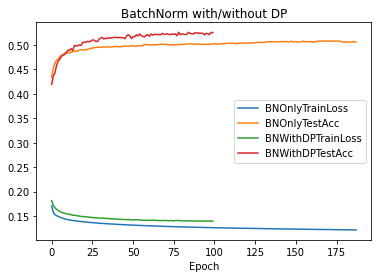
\includegraphics[scale=0.5]{Figures/7.BatchNorm/with-without dp}
    \caption{Performance of models with/without Dropout}
\end{figure}

    It can be seen that DP will be better if work with BatchNorm layer.
    Another found is that Batchnorm without dropout will greatly reduce the converging speed and lower the running speed.
    This reveals another important function of Dropout, which is reducing the workload of both forward/backward proporgation.

\section{Discussion and Conclusion}
    In this task, an understanding of the underlying logic of deep learning was gained by implementing a multi-classifier from scratch.

    The implemented multi-classifier has been experimented with several times, applying well-established techniques
    and substituting different hyperparameters, without obtaining satisfactory results,
    and the reasons for this are worth considering.
    One possible reason for this is that the decision boundaries
    between the different categories in the dataset intersect, resulting in the model not learning each category correctly.
    From this persepctive, it reveals a very important fact, which is that all amazing machine learning techniques are
    based on data, and only when the quality and quantity of the data is high enough can the model achieve a good performance.

    From some noteworthy experiments, it has been observed that a slight change on some hyper-parameters will have a
    very significant impact on the performance of the model, like learning rate.
    Also observed is the power of certain machine learning techniques, such as dropout, to mitigate overfitting while improving the speed of training.
    This indicated that care should be taken when choosing hyperparameters,
    and the best way to get the best set of hyperparameters is through continuous experimentation.




\section{Appendix}
\subsection{Manual}
    The module implementation has been finished in a form of python package named "dl" in the directory "dl" of the project root.

    The best model is trained in the model.ipynb in the root of this project.
    It can be directly opened in jupyter lab/notebook and run in the same directory with the package (if the package has not been installed).
    You can use it as the sample of your own usage.
\subsubsection{Prerequests}
    python $\geq$ 3.8, Numpy $\geq$ 1.22 and Scipy $\geq$ 1.8

    A lower version pakage is likely to be working, but not guarenteed.

\subsubsection{Setup(optional)}
    If an installation is prefered, run the following code in the root of this project to install the package:

\begin{lstlisting}
    cd /path/to/package/and/setup.py
    pip install .
\end{lstlisting}

\subsubsection{importing}
    There are 3 options to use this package.

    If the package has been installed:
    \begin{lstlisting}
    import dl
    \end{lstlisting}
    at the top of your python script directly.

    If the package has not been installed, you may add following lines to use the package:
    \begin{lstlisting}
    import sys
    sys.path.append("path/to/package")
    import dl
    \end{lstlisting}

    Or if you create any python script under the root of this project, you can import the package directly as well.

\subsubsection{Usage}
    For detailed usage, checkout the comment or run:
    \begin{lstlisting}
    pydoc -p [port]
    \end{lstlisting}
    in the command line. Replace [port] by your preference. Then open the website "localhost:[port]", search for
    package "dl".

    To train a model:
\begin{enumerate}
    \item Read your data set, preprocess them.
    \item Construct a dl.dataset.Dataset object by your data set.
    \item Construct a dl.nn.Module object to define your network structure and forward behaviour.
    \item Define an optimizer using classes in dl.optimizer. You may define your own by inherit class dl.optimizer.Optim.
    \item Define a lossfunction using classes in dl.metrics. You may define your own by inherit class dl.metrics.LossFunction.
    \item Define you training process. For each iteration of your training, you should:
    \begin{enumerate}
        \item Call the model object to process feature data, get the returned yhat.
        \item Call the loss function with yhat and ground truth to calculate the loss.
        \item Call the loss.backward() to perform a back proporgation.
        \item Call the optimizer.step() to update the parameters.
    \end{enumerate}
\end{enumerate}

\end{document}